\documentclass{article}
\usepackage[utf8]{inputenc}
\usepackage{amsmath, amssymb, amsthm}
\usepackage{geometry}
\usepackage{microtype}
\usepackage{booktabs}
\usepackage[ngerman]{babel}
\usepackage{setspace}
\usepackage{graphicx}

% Anpassen der Seitenränder
\geometry{left=25mm, right=25mm, top=25mm, bottom=25mm}

% Einstellen des Zeilenabstandes
\setstretch{1.25}

\title{Lösungen zu Übungsaufgaben 07 \\ \small Gruppe: Mi 08-10 SR 2, Barbara Rieß}
\author{Linus Keiser}
\date{13. Dezember 2023}

% Theorem-Umgebungen
\renewcommand{\proofname}{Beweis}
\newtheorem{theorem}{Satz}
\theoremstyle{definition}
\newtheorem{definition}{Definition}
\theoremstyle{remark}
\newtheorem*{remark}{Bemerkung}

\begin{document}

\graphicspath{ {./ } }

\maketitle
\section*{Aufgabe 25}

\subsection*{(a) Betragssummennorm}

\textit{Zu zeigen:} die Abbildung \( \| x \|_1 := \sum_{k=1}^{n} |x_k| \) für \( x = (x_1, \ldots, x_n)^T \in \mathbb{R}^n \) eine Norm auf \( \mathbb{R}^n \) definiert.

\begin{proof} Wir überprüfen die Normeigenschaften (N1) bis (N4).

    \textbf{(N1) Positivität:}
    Da der Betrag einer jeden reellen Zahl nichtnegativ ist, folgt, dass die Summe der Beträge der Komponenten von \( x \) ebenfalls nichtnegativ ist. Daher gilt \( \| x \|_1 \geq 0 \) für alle \( x \in \mathbb{R}^n \).

    \textbf{(N2) Definitheit:}
    Es gilt \( \| x \|_1 = 0 \) genau dann, wenn jeder Betrag \( |x_k| = 0 \) für \( k = 1, \ldots, n \) ist. Dies ist genau dann der Fall, wenn jedes \( x_k = 0 \) ist. Daher ist \( \| x \|_1 = 0 \) genau dann, wenn \( x = 0 \).

    \textbf{(N3) Homogenität:}
    Für ein beliebiges \( \alpha \in \mathbb{R} \), betrachten wir \( \| \alpha x \|_1 = \sum_{k=1}^{n} |\alpha x_k| \). Aufgrund der Eigenschaften des Betrags gilt \( |\alpha x_k| = |\alpha||x_k| \). Daher ist \( \| \alpha x \|_1 = |\alpha| \sum_{k=1}^{n} |x_k| = |\alpha| \| x \|_1 \).

    \textbf{(N4) Dreiecksungleichung:}
    Für \( x, y \in \mathbb{R}^n \), gilt \( \| x + y \|_1 = \sum_{k=1}^{n} |x_k + y_k| \). Aufgrund der Dreiecksungleichung für Beträge folgt \( |x_k + y_k| \leq |x_k| + |y_k| \). Daher ist \( \| x + y \|_1 \leq \sum_{k=1}^{n} (|x_k| + |y_k|) = \| x \|_1 + \| y \|_1 \).

    Damit sind die Normeigenschaften für \( \| x \|_1 \) gezeigt.
\end{proof}

\subsection*{(b) Maximumsnorm}

\textit{Zu zeigen:} die Abbildung \( \| x \|_{\infty} := \max \{ |x_1|, |x_2|, \ldots, |x_n| \} \) für \( x = (x_1, \ldots, x_n)^T \in \mathbb{R}^n \) eine Norm auf \( \mathbb{R}^n \) definiert.

\begin{proof} Hierbei überprüfen wir erneut die Normeigenschaften (N1) bis (N4).

    \textbf{(N1) Positivität:}
    Das Maximum einer Menge nichtnegativer Zahlen ist nichtnegativ. Da die Beträge der Komponenten von \( x \) nichtnegativ sind, folgt, dass \( \| x \|_{\infty} \geq 0 \) für alle \( x \in \mathbb{R}^n \).

    \textbf{(N2) Definitheit:}
    Wenn \( \| x \|_{\infty} = 0 \), dann ist das Maximum der Beträge der Komponenten von \( x \) null. Dies bedeutet, dass jede Komponente \( x_k \) null sein muss, und somit ist \( x = 0 \).

    \textbf{(N3) Homogenität:}
    Für ein beliebiges \( \alpha \in \mathbb{R} \), betrachten wir \( \| \alpha x \|_{\infty} \). Es gilt \( \| \alpha x \|_{\infty} = \max \{ |\alpha x_1|, ..., |\alpha x_n| \} = |\alpha| \max \{ |x_1|, ..., |x_n| \} = |\alpha| \| x \|_{\infty} \), was aus den Eigenschaften des Betrags folgt.

    \textbf{(N4) Dreiecksungleichung:}
    Für \( x, y \in \mathbb{R}^n \) gilt \( \| x + y \|_{\infty} = \max \{ |x_1 + y_1|, ..., |x_n + y_n| \} \). Unter Anwendung der Dreiecksungleichung für Beträge ergibt sich \( |x_k + y_k| \leq |x_k| + |y_k| \). Daher ist \( \| x + y \|_{\infty} \leq \max \{ |x_k| + |y_k|, ..., |x_n| + |y_n| \} \). Da für jede Komponente gilt, dass \( |x_k|, |y_k| \leq \| x \|_{\infty}, \| y \|_{\infty} \), folgt, dass \( \| x + y \|_{\infty} \leq \| x \|_{\infty} + \| y \|_{\infty} \).

    Damit sind die Normeigenschaften (N1) bis (N4) für \( \| x \|_{\infty} \) gezeigt.
\end{proof}


\section*{Aufgabe 26}

\textit{Ziel:} Umformung in die Form \( z = x + iy \) und Berechnung von Realteil, Imaginärteil und Betrag.

\subsubsection*{(a) \( z = (3 + 4i)(2 - i)^{2} - (5 - i) + 27\)}

Zunächst erweitern wir den quadratischen Term \((2 - i)^{2}\). Unter Verwendung der binomischen Formel und der Eigenschaft \(i^2 = -1\) gilt:
\begin{align*}
    (2 - i)^2 & = (2 - i)(2 - i)                \\
              & = 2^2 - 2 \cdot 2 \cdot i + i^2 \\
              & = 4 - 4i - 1                    \\
              & = 3 - 4i.
\end{align*}
Durch Multiplikation mit dem verbundenen Term \( (3 + 4i) \) erhalten wir folglich:
\begin{align*}
    (3 + 4i)(3 - 4i) & = (3 + 4i) \cdot (3 - 4i) \\
                     & = 25.
\end{align*}
Zusammen mit den anderen Termen ergibt sich:
\begin{align*}
    z & = 25 - (5 - i) + 27 \\
      & = 25 - 5 + i + 27   \\
      & = 47 + i.
\end{align*}
Daher ist der Realteil \( x = 47 \), der Imaginärteil \( y = 1 \) und der Betrag von \( z \) ist \( |z| = \sqrt{47^2 + 1^2} = \sqrt{2210} \).

\subsubsection*{(b) \( z = \frac{7 - 3i}{6i - 4} \)}

Wir vereinfachen den Bruch durch Multiplikation von Zähler und Nenner mit der konjugierten Zahl des Nenners. Dies führt zu einem reellen Nenner. Die konjugierte Zahl zu \( 6i - 4 \) ist
\begin{align*}
    \text{Konjugierte: } & 6i - 4 \rightarrow -6i - 4.
\end{align*}
Damit ist der vereinfachte Bruch
\begin{align*}
    z & = \frac{7 - 3i}{6i - 4} \cdot \frac{-6i - 4}{-6i - 4} \\
      & = \frac{(7 - 3i)(-6i - 4)}{(6i - 4)(-6i - 4)}         \\
      & = \frac{-46 - 30i}{52}.
\end{align*}
Durch Kürzen erhalten wir:
\begin{align*}
    z & = -\frac{23}{26} - \frac{15i}{26}.
\end{align*}
Daher ist der Realteil \( x = -\frac{23}{26} \), der Imaginärteil \( y = -\frac{15}{26} \) und der Betrag von \( z \) ist \( |z| = \sqrt{\left(-\frac{23}{26}\right)^2 + \left(-\frac{15}{26}\right)^2} \).

\section*{Aufgabe 27}

\subsection*{(a)}
Wir zeigen, dass für alle \( z, w \in \mathbb{C} \) die Regel \( \overline{z + w} = \overline{z} + \overline{w} \) gilt.

\proof Es sei
\begin{enumerate}
    \item	\( z = x + yi \), wobei \( x \) der Realteil und \( y \) der Imaginärteil von \( z \) ist (und \( i \) die imaginäre Einheit).
    \item	\( w = u + vi \), wobei \( u \) der Realteil und \( v \) der Imaginärteil von \( w \) ist.
\end{enumerate}
Wir berechnen die linke und rechte Seite der Gleichung \( \overline{z + w} = \overline{z} + \overline{w} \) und zeigen, dass beide Seiten identisch sind.
Für die linke Seite gilt:
\[ z + w = (x + yi) + (u + vi) = (x + u) + (y + v)i. \]
Dann ist \( \overline{z + w} = \overline{(x + u) + (y + v)i} = (x + u) - (y + v)i \). Für die rechte Seite \( \overline{z} + \overline{w} \) gilt:
\begin{align*}
    \overline{z} + \overline{w} & = \overline{x + yi} + \overline{u + vi} \\
                                & = x - yi + u - vi                       \\
                                & = (x + u) - (y + v)i.
\end{align*}
Wir sehen, dass die linke und rechte Seite identisch sind. Daher ist die Gleichung \( \overline{z + w} = \overline{z} + \overline{w} \) für alle \( z, w \in \mathbb{C} \) wahr.
\endproof

\subsection*{(b)}
Wir zeigen, dass für alle \( z, w \in \mathbb{C} \) die Regel \( \overline{z \cdot w} = \overline{z} \cdot \overline{w} \) gilt.

\proof Es gelte die Definition von \( z \) und \( w \) wie in (a). Wir berechnen die linke und rechte Seite der Gleichung \( \overline{z \cdot w} = \overline{z} \cdot \overline{w} \) und zeigen, dass beide Seiten identisch sind.
Zuerst berechnen wir wir:
\begin{align*}
    z \cdot w & = (x + yi) \cdot (u + vi)                                        \\
              & = xu + xvi + yiu + yvi^2                                         \\
              & = (xu - yv) + (xv + yu)i. \quad \text{Da } i^2 = -1 \text{ ist.}
\end{align*}
Dann ist
\begin{align*}
    \overline{z \cdot w} & = \overline{(xu - yv) + (xv + yu)i} \\
                         & = (xu - yv) - (xv + yu)i.
\end{align*}
Für die rechte Seite \( \overline{z} \cdot \overline{w} \) gilt:
\begin{align*}
    \overline{z} \cdot \overline{w} & = \overline{x + yi} \cdot \overline{u + vi} \\
                                    & = x - yi \cdot u - vi                       \\
                                    & = xu - xvi - yui + yvi^2                    \\
                                    & = (xu - yv) - (xv + yu)i.
\end{align*}
Wir sehen, dass die linke und rechte Seite identisch sind. Daher ist die Gleichung \( \overline{z \cdot w} = \overline{z} \cdot \overline{w} \) für alle \( z, w \in \mathbb{C} \) wahr.
\endproof

\subsection*{(c)}
Wir zeigen, dass für alle \( z \in \mathbb{C} \) die Regel \( z + \overline{z} = 2 \operatorname{Re}(z) \) gilt.

\proof Es gelte die Definition von \( z \) wie in (a).
Das komplex Konjugierte von \( z \) ist \( \overline{z} = x - yi \). Dann ist
\begin{align*}
    z + \overline{z} & = (x + yi) + (x - yi) \\
                     & = 2x.
\end{align*}
Der Realteil von \( z \) ist \( x \), also ist \( 2x = 2 \operatorname{Re}(z) \). Daher ist die Gleichung \( z + \overline{z} = 2 \operatorname{Re}(z) \) für alle \( z \in \mathbb{C} \) wahr.
\endproof

\subsection*{(d)}
Wir zeigen, dass für alle \( z \in \mathbb{C} \) die Regel \( z - \overline{z} = 2i \operatorname{Im}(z) \) gilt.

\proof Es gelte die Definition von \( z \) wie in (a).
Das komplex Konjugierte von \( z \) ist \( \overline{z} = x - yi \). Dann ist
\begin{align*}
    z - \overline{z} & = (x + yi) - (x - yi) \\
                     & = 2yi.
\end{align*}
Der Imaginärteil von \( z \) ist \( y \), also ist \( 2yi = 2i \operatorname{Im}(z) \). Daher ist die Gleichung \( z - \overline{z} = 2i \operatorname{Im}(z) \) für alle \( z \in \mathbb{C} \) wahr.
\endproof

\subsection*{(e)}
Wir zeigen, dass für alle \( z \in \mathbb{C} \) die Regel \( z \overline{z} \ge 0 \) und \( z \overline{z} = 0 \leftrightarrow z = 0\) gilt.

\proof Es gelte wieder die Definition von \( z \) wie in (a).
Für \( z \overline{z} \) gilt:
\begin{align*}
    z \overline{z} & = (x + yi)(x - yi) \\
                   & = x^2 + y^2.
\end{align*}
Wir wissen, dass \( z \overline{z} \ge 0\), weil sowohl \( x^2 \) als auch \( y^2 \) als Quadrate reeler Zahlen immer positiv sind, also ist auch die Summe \( x^2 + y^2 \ge 0 \).
Für die Bedingung der Äquivalenz gilt für die Hinrichtung, dass wenn \( z \overline{z} = 0 \) ist, dann muss \( x^2 + y^2 = 0\) sein. Da Quadrate nur dann null sind, wenn die Basis null ist, folgt \( x = 0 \) und \( y = 0 \). Also ist \( z = 0 \).
Für die Rückrichtung gilt, dass wenn \( z = 0 \) ist, dann ist offensichtlich \( x = 0 \) und \( y = 0 \), und somit ist\( z \overline{z} = x^2 + y^2 = 0 \).
Damit haben wir gezeigt, dass \( z \overline{z} \) immer nichtnegativ ist und nur dann null wird, wenn \( z \) selbst null ist.
\endproof

\section*{Aufgabe 28}

\subsection*{(a) i}

\textbf{Satz.} Es gilt \( z^n = |z|^n(\cos(n \varphi) + i \sin(n \varphi))\) für alle \( z = |z|(\cos(\varphi) + i \sin(\varphi)) \in \mathbb{C} \) und \( n \in \mathbb{N} \).

\begin{proof} Gegeben ist \( z = |z|(\cos(\varphi) + i\sin(\varphi)) \) in der Polarform.

    Wir wollen \( z^ n \) bestimmen. Da \( z \) in Polarform vorliegt können wir die Moivre'sche Formel anwenden, die besagt, dass \( (r(\cos(\theta) + i\sin(\theta)))^n = r^n(\cos(n\theta) + i\sin(n\theta)) \) für jedes \( r \in \mathbb{R} \) und \( \theta \in \mathbb{R} \). In unserem Fall ist dann In unserem Fall ist \( r = |z| \) und \( \theta = \varphi \).

    Durch einsetzen der Werte in die Moivre'sche Formel erhalten wir:
    \[ z^n = (|z|(\cos(\varphi) + i\sin(\varphi)))^n = |z|^n(\cos(n\varphi) + i\sin(n\varphi)) \]
    Das ist genau die Formel, die wir zeigen wollten. Damit ist der Satz bewiesen.
\end{proof}

\subsection*{(a) ii}

\textbf{Satz.} Es gilt \( z_{k,n}^n = 1 \) für alle \( k \in \{0, \ldots, n - 1\} \).

\begin{proof} Gegeben ist \( z_{k,n} = \cos\left(\frac{2\pi k}{n}\right) + i\sin\left(\frac{2\pi k}{n}\right) \), eine Darstellung von \( z_{k,n} \) in der Polarform, mit dem Betrag \( |z_{k,n}| = 1 \) (da Kosinus und Sinus auf dem Einheitskreis liegen) und dem Argument \( \varphi = \frac{2\pi k}{n} \). Wie zuvor nutzen wir die Moivre'sche Formel. Für \( z^n \), wobei \( z = |z|(\cos(\varphi) + i\sin(\varphi)) \), gilt \( z^n = |z|^n(\cos(n\varphi) + i\sin(n\varphi)) \). Für \( z_{k,n} \) wird dies zu \( z_{k,n}^n = (\cos\left(\frac{2\pi k}{n}\right) + i\sin\left(\frac{2\pi k}{n}\right))^n \).
    Für \( z_{k,n}^n \) gilt dann:
    \[ z_{k,n}^n = \left(\cos\left(\frac{2\pi k}{n}\right) + i\sin\left(\frac{2\pi k}{n}\right)\right)^n = \cos(2\pi k) + i\sin(2\pi k). \]
    Ferner ist \( \cos(2\pi k) = 1 \) und \( \sin(2\pi k) = 0 \), da \( 2\pi k \) ein ganzzahliges Vielfaches von \( 2\pi \) ist, und der Kosinus und Sinus von ganzzahligen Vielfachen von \( 2\pi \) sind jeweils 1 bzw. 0.
    Daher ist \( z_{k,n}^n = 1 \) für alle \( k \in \{0, \ldots, n - 1\} \).
\end{proof}

\subsection*{(b)}

Wir berechnen zunächst die Punkte \( z_{k,4}\) mit der algemeinen Formel \( z_{k,n} = \cos(\frac{2 \pi k}{n}) + i \sin(\frac{2 \pi k}{n})\). Für \( n = 4 \) und \( k = 0, 1, 2, 3 \) erhalten wir:
\begin{align*}
    z_{0,4} & = \cos \left( \frac{2 \pi \cdot 0}{4} \right) + i \sin \left( \frac{2 \pi \cdot 0}{4} \right) \\
    z_{1,4} & = \cos \left( \frac{2 \pi \cdot 1}{4} \right) + i \sin \left( \frac{2 \pi \cdot 1}{4} \right) \\
    z_{2,4} & = \cos \left( \frac{2 \pi \cdot 2}{4} \right) + i \sin \left( \frac{2 \pi \cdot 2}{4} \right) \\
    z_{3,4} & = \cos \left( \frac{2 \pi \cdot 3}{4} \right) + i \sin \left( \frac{2 \pi \cdot 3}{4} \right)
\end{align*}
Die Menge \( K \) ist der Einheitskreis in der komplexen Ebene, definiert durch \( K = \{(x,y) \in \mathbb{R}^2 : x^2 + y^2 = 1\} \). Der Einheitskreis \( K \) ist definiert als die Menge aller Punkte in der Ebene, deren Entfernung vom Ursprung genau 1 ist, was durch die Gleichung \( x^2 + y^2 = 1 \) ausgedrückt wird.
Die Punkte \( z_{k,4} \) werden auf dem Einheitskreis \( K \) liegen, da \( |z_{k,4}| = 1 \) für alle \( k \). Sie repräsentieren die vierten Einheitswurzeln und sind durch ihre Winkel \( \frac{2 \pi k}{4} \) für \( k = 0, 1, 2, 3 \) bestimmt.
\begin{itemize}
    \item \( z_{0,4} \) liegt bei \( (1,0) \),
    \item \( z_{1,4} \) bei \( (0,1) \),
    \item \( z_{2,4} \) bei \( (-1,0) \),
    \item \( z_{3,4} \) bei \( (0,-1) \).
\end{itemize}
Damit ergibt sich folgende Darstellung der Punkte \( z_{k,4} \) in der komplexen Ebene:

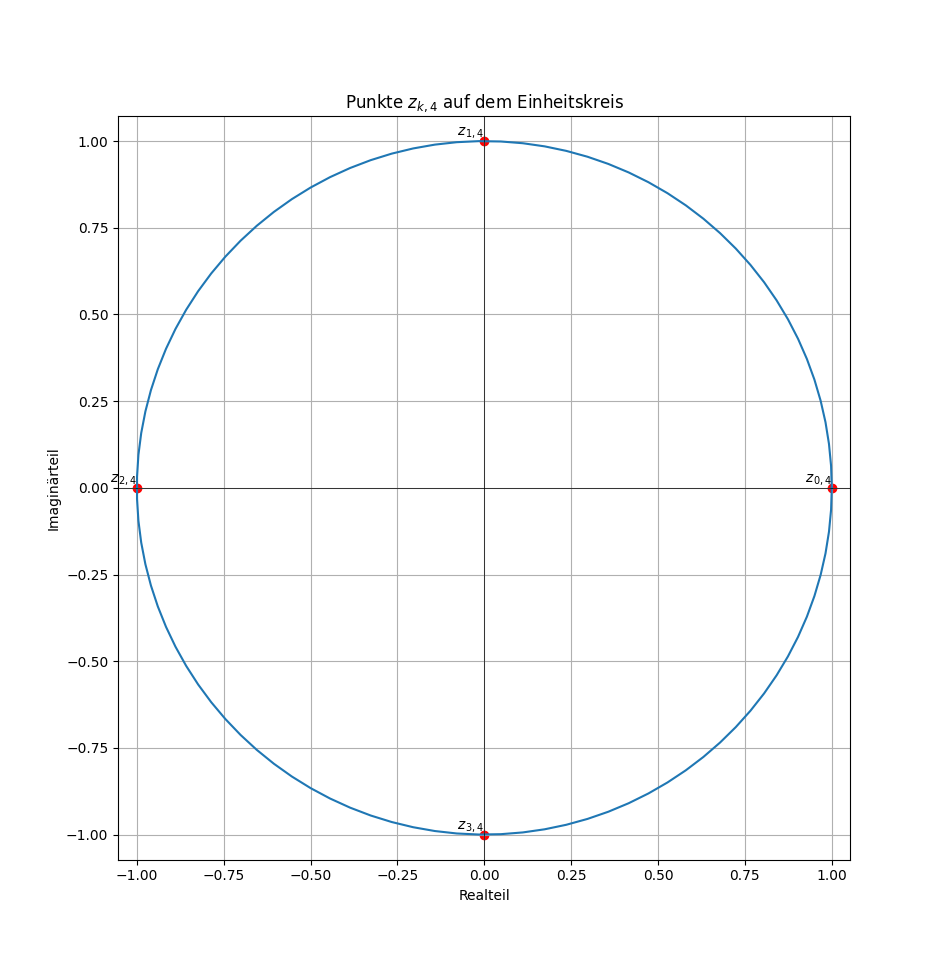
\includegraphics[scale=0.6]{Figure_1.png}

\end{document}




